\subsection{单链平均和算子}
在前面的章节中,我们描述了如何使用Chapman-Kolmogorov或Fokker-Planck方程计算单链在外场存在下的分布函数。单链配分函数和约化分布函数(链传播子)是非均匀聚合物理论中的中心对象,有必要将其它“可观测”量表示为外场变量的显式泛函。这主要的量与单链自由度构象全体平均受到外势有关。例如:离散高斯链受到化学势$w (\mathbf{r})$的情况下,我们可以定义任何函数$f(\mathbf{r}^{N+1})$珠坐标(bead coordinates)的单链平均:
\begin{equation}\label{3.46}
<f(\mathbf{r}^{N+1})>_{[w]}= \frac{\int  f(\mathbf{r}^{N+1})~\exp[-\beta U(\mathbf{r}^{N+1})]~d \mathbf{r}^{N+1}}{\int \exp[-\beta U(\mathbf{r}^{N+1})]~d\mathbf{r}^{N+1}}
\end{equation}

其中$U(\mathbf{r}^{N+1})$是公式(\ref{3.1})给出的电势。尖括号的下标$[w]$在对珠坐标进行平均,平均量可以看作是外场$w(\mathbf{r})$的函数。同样,对于存在化学势和应变场$w(\mathbf{r})$和$\mathbf{\epsilon}$的连续高斯链,相应的单链平均值可以定义为:
\begin{equation}\label{3.47}
<f[\mathbf{r}]>_{[w ,\epsilon]}=\frac{\int f[\mathbf{r}]~\exp(-\beta U_{0}[\mathbf{r}]-\beta U_{1}[\mathbf{r},w]-\beta U_{el}[\mathbf{r},\epsilon])~D\mathbf{r}}{\int \exp(-\beta U_{0}[\mathbf{r}]-\beta U_{1}[\mathbf{r},w]-\beta U_{el}[\mathbf{r},\epsilon])~D\mathbf{r}}
\end{equation}
其中$f[\mathbf{r}]$是链构型$\mathbf{r}(s)$的任意泛函。

主要有趣的单链平均量是段密度、密度相关性和弹性应力,所有这些都可以与非均匀聚合物实验中的可观测值联系起来。我们将看到在某些情况,可以通过取关于场变量$w(\mathbf{r})$和$\mathbf{\epsilon}$的规范配分函数$Q[w]$和$Q[w,\epsilon]$的函数导数来获得这些结果。读者不熟悉函数的变分,建议参考附录C。
\subsubsection{密度算子}
首先,我们考虑在化学势$w(\mathbf{r})$作用下的单个柔性聚合物的平均段数密度的计算问题。这个数量定义为:
\begin{equation}\label{3.48}
\rho(\mathbf{r};[w])\equiv<\tilde{\rho}(\mathbf{r})>_{[w]}
\end{equation}

其中微观密度$\tilde{\rho}(\mathbf{r})$由公式(\ref{3.3})或(\ref{3.18})给出,这取决于采用的是离散的或连续的高斯链模型。我们将$\rho(\mathbf{r};[w])$称为单链密度算子,因为它将平均段密度表示为强加场$w$的一个泛函。我们将在第四章中看到,场构造分布合适时,许多聚合物相互作用流体的平均单体密度与算子$\rho(\mathbf{r};[w])$的平均值成正比。在这种情况下场不是外部强加的,而是由非键单体之间的相互作用在内部产生的。因此,在多链流体中的“可观测”量的计算将涉及两种不同类型全体平均:(i)公式(\ref{3.46})和(\ref{3.47})描述单链的平均;(ii)内部产生电势场分布的场论平均值。关于第二类平均的讨论将推迟到第四章。

在计算公式(\ref{3.48})时,我们再次指出$w(\mathbf{r})$和$\tilde{\rho}(\mathbf{r})$是热力学共轭变量。因此,$-lnQ[w]$泛函关于$w(\mathbf{r})$的导数会生成单链$\tilde{\rho}(\mathbf{r})$的平均。例如:在离散高斯链的情况下,关于$Q$的公式(\ref{3.4})和单链平均定义(\ref{3.46})。特别是:
\begin{equation}\label{3.49}
-\frac{\delta~lnQ[w]}{\delta w(\mathbf{r})}=-\frac{1}{Q[w]}\frac{\delta Q[w]}{\delta w(\mathbf{r})}=<\tilde{\rho}(\mathbf{r})>_{[w]}
\end{equation}
因此,段密度算子的另一个表达式是
\begin{equation}\label{3.50}
\rho(\mathbf{r};[w])=-\frac{1}{Q[w]}\frac{\delta Q[w]}{\delta w(\mathbf{r})}
\end{equation}

这个表达式的右边可以通过公式(\ref{3.6})的泛函微分直接计算(对于离散的高斯链)。这导致:
\begin{align}\label{3.51}
\begin{split}
\frac{\delta Q[w]}{\delta w(\mathbf{r})}=\frac{1}{V}\sum_{j=0}^{N}\int &[e^{-w(\mathbf{r}_{N})}\Phi(\mathbf{r}_{N}-\mathbf{r}_{N-1})e^{-w(\mathbf{r}_{N-1})}\Phi(\mathbf{r}_{N-1}-\mathbf{r}_{N-2}) \\ &\times \ldots e^{-w(\mathbf{r}_{j})}(-1)\delta(\mathbf{r}-\mathbf{r}_j)\Phi(\mathbf{r}_j-\mathbf{r}_{j-1})e^{-w(\mathbf{r}_j-1)}\\ & \times \ldots e^{-w(\mathbf{r}_{2})}\Phi(\mathbf{r}_{2}-\mathbf{r}_{1})e^{-w(\mathbf{r}_{1})}\Phi(\mathbf{r}_{1}-\mathbf{r}_{0})e^{-w(\mathbf{r}_{0})}]~d\mathbf{r}^{N+1}
\end{split}
\end{align}
公式(\ref{3.51})中的δ函数可以用来消去$\mathbf{r}_{j}$上的积分,即珠 j的位置。这产生了表因式分解的表达示,类似于公式(\ref{3.10})描述的的因式分解性质,如图3.1所示。按照同样的推理,可以通过组成传播子$q(\mathbf{r},j;[w])$重写公式(\ref{3.51}),用“互补”传播子$q(\mathbf{r},N-j;[w])$描述链段的统计权重,该链段从珠0开始,终止于珠j。后者描述的统计权重与剩余链段相关,从珠N开始,用珠j完成。因此,公式(\ref{3.51})可以表示为:
\begin{equation}\label{3.52}
\frac{\delta Q[w]}{\delta w(\mathbf{\mathbf{\mathbf{r}}})}=-\frac{e^{w(\mathbf{r})}}{V}\sum_{j=0}^{N}~q(\mathbf{r},N-j;[w])~q(\mathbf{r},j;[w])
\end{equation}
因此:	
\begin{equation}\label{3.53}
\rho(\mathbf{r},[w])=\frac{e^{w}}{VQ[w]}\sum_{j=0}^{N}~q(\mathbf{r},N-j;[w])~q(\mathbf{r},j;[w])
\end{equation}

方程(\ref{3.53})是非均匀聚合物理论中的一个重要公式,因为它提供了计算具有任意电势$w(\mathbf{r})$的离散高斯链平均段密度的方法。给出$w(\mathbf{r})$的表达式,首先递归求解公式(\ref{3.8})[在初始条件(\ref{3.7})下],得到j=0,1,2,…,N的$q(\mathbf{r},j;[w])$。其次,用公式(\ref{3.54})计算$Q[w]$。这些结果可用于计算公式(\ref{3.53})右侧的表达式。因此,对所有珠子j的链传播子$q(\mathbf{r},j;[w])$的知识足以确定规范化配分函数$Q[w]$和平均段密度$\rho(\mathbf{r};[w])$。

这些结果很容易推广到其他链模型中。按照公式(\ref{3.21})离散的连续高斯链,连续高斯链类似公式(\ref{3.53})的模拟量是:
\begin{align}\label{3.54}
\begin{split}
\rho(\mathbf{r},[w])&=-\frac{1}{Q[w]}\frac{\delta Q[w]}{\delta w(\mathbf{r})}\\ &=\frac{\triangle s ~\exp[\triangle sw(\mathbf{r})]}{VQ[w]}\sum_{j=0}^{N_s}~q(\mathbf{r},(N_s-j)\triangle s;[w])~q(\mathbf{r},j\triangle s;[w])
\end{split}
\end{align}
当取连续极限$N_s\to \infty$,$\triangle s=N/N_s\to 0$,时,我们发现这个表达式可以化简为:
\begin{equation}\label{3.55}
\rho(\mathbf{r},[w])=\frac{1}{VQ[w}\int_{0}^{N}q(\mathbf{r},(N-s);[w])~q(\mathbf{r},s;[w])~ds
\end{equation}
这是一个众所周知的结果,是非均匀聚合物的核心理论。其次,我们发现它和连续高斯链(\ref{3.27})的因式分解性质相似。

密度算子$\rho(\mathbf{r},[w])$描述了链段的平均密度,而不是它们沿聚合物的位置。另一个有用的密度算子,例如:连续高斯链是数量:
\begin{equation}\label{3.56}
\rho(\mathbf{r},s;[w])\equiv <\tilde{\rho}(\mathbf{r},s)>_{[w]}
\end{equation}
表示位于等高线位置s的分段的平均密度。用$\tilde{\rho}(\mathbf{r},s)=\delta(\mathbf{r}-\mathbf{r}(s))$表示各段在位置s的微观密度。通过引入共轭场$\omega_s(\mathbf{r})$来计算$\tilde{\rho}(\mathbf{r},s)$
,仅能计算单体s,并对相互作用能贡献一个附加项:
\begin{equation}\label{3.57}
\beta U_1[\mathbf{r},w ,w_s]=\int [\tilde{\rho}(\mathbf{r}^{'})w (\mathbf{r}^{'})+\tilde{\rho}(\mathbf{r}^{'},s)w_s(\mathbf{r}^{'})]~d\mathbf{r}^{'}
\end{equation}
下面的参数类似于公式(\ref{3.50})的参数,给出结果:
\begin{equation}\label{3.58}
\rho(\mathbf{r},s;[w])=<\tilde{\rho}(\mathbf{r},s)>_{[w]}
=-\frac{\delta~lnQ[w,w_s]}{\delta w_s(\mathbf{r})} \bigg |_{w_s=0}
\end{equation}
我们现回到$Q[w,w_s]$的路径积分离散化的步骤,对$w_s$微分,并取连续极限。如果令$w_s(\mathbf{r})=0$,结果是:
\begin{equation}\label{3.59}
\rho(\mathbf{r},s;[w])=\frac{1}{VQ[w]}~q(\mathbf{r},(N-s);[w])~q(\mathbf{r},s;[w])
\end{equation}

图\ref{figure1}描述了公式(\ref{3.59})的物理含量,与公式(\ref{3.55})的比较,我们发现平均总段密度$\rho(\mathbf{r};[w])$是所有轮廓位置$0\le s\le N$上的平均段s的密度$\rho(\mathbf{r},s;[w])$的简单积分:

\begin{figure}[H]
\centering
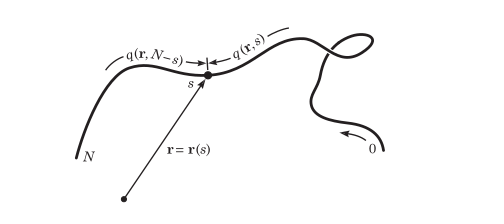
\includegraphics[width=15cm]{./figures/32.png}
\caption{说明位于连续高斯链位置s处的段的平均密度的组成公式(\ref{3.59})。轮廓长度s的链段的统计权重$q(\mathbf{r},s;[w])$在点$r=r(s)$处与具有轮廓长度$N−s$的基本链段的统计权重$q(\mathbf{r},N−s;[w])$连接。}
\label{figure1}
\end{figure}

\begin{equation}\label{3.60}
\rho(\mathbf{r};[w])=\int_{0}^{N}\rho(\mathbf{r},s;[w])~ds
\end{equation}
该公式与微观密度$\tilde{\rho}(\mathbf{r})$和$\tilde{\rho}(\mathbf{r},s)$之间的关系有明显的一致性。

公式(\ref{3.59})的一个特例是特别令人感兴趣的。通过设置$s=0$或$s=N$,可以得到链端段的平均密度。在目前的均聚物的情况下,两个链端是不可区分的,所以总链端密度可以由
\begin{align}\label{3.61}
\begin{split}
\rho_e(\mathbf{r};[w])&\equiv \rho(\mathbf{r},0;[w])+\rho(\mathbf{r},N;[w])\\  &=\frac{2}{VQ[w]}~q(\mathbf{r},N;[w])
\end{split}
\end{align}
在这个表达式的第二行中,我们使用了$q(\mathbf{r},0;[w])=1$。因此,在应用规范化$\frac{2}{VQ[w]}$后,传播子$q(\mathbf{r},N;[w])$可以解释为链端在r位置的平均密度。

公式(\ref{3.65})-(\ref{3.61})中的结果可以很容易地推广到离散高斯链模型。为了简洁起见,我们省略简结的概括,转而转向类似蠕虫的链。在类虫链模型,引入了一个场$w(\mathbf{r},\mathbf{u})$,它与片段位置和取向的微观密度$\tilde{\rho}(\mathbf{r},\mathbf{u})$的共轭。因此,对于段位置和取向密度的单链平均值的算子可以被定义为:
\begin{equation}\label{3.62}
\rho(\mathbf{r},\mathbf{u};[w])\equiv <\tilde{\rho}(\mathbf{r},\mathbf{u})>_{[w]}=-\frac{\delta lnQ[w]}{\delta w(\mathbf{r},\mathbf{u})}
\end{equation}
这个表达式可以通过离散$Q[w]$的路径积分、对$w(r,u)$的微分和恢复连续极限来计算。结果如下:
\begin{equation}\label{3.63}
\rho(\mathbf{r},\mathbf{u};[w])=\frac{1}{4\pi VQ[w]}\int_{0}^{L_c} q(\mathbf{r},-\mathbf{u},L_c-s;[w])~q(\mathbf{r},\mathbf{u},s;[w])~ds
\end{equation}
这个表达式类似于因式分解性质(\ref{3.41}),因为传播子$q(\mathbf{r},-u,L_c-s,[w])$描述了“互补”链段的统计权重,其符号为u相反数。

从公式(\ref{3.63})中可以得到几个相关的平均密度。在r或u的两边积分后,得到段方向或位置的平均密度。因此,
\begin{align}\label{3.64}
\begin{split}
\rho(\mathbf{u};[w])&\equiv\int \rho(\mathbf{r},\mathbf{u};[w])~d\mathbf{r} \\&=\frac{1}{4\pi VQ[w]}\int  \int_{0}^{L_c}q(\mathbf{r},-\mathbf{u},L_c-s;[w])~q(\mathbf{r},\mathbf{u},s;[w])~d\mathbf{r}ds
\end{split}
\end{align}
和
\begin{align}\label{3.65}
\begin{split}
\rho(\mathbf{r};[w])&\equiv\int \rho(\mathbf{r},\mathbf{u};[w])~d\mathbf{u} \\&=\frac{1}{4\pi VQ[w]}\int  \int_{0}^{L_c}q(\mathbf{r},-\mathbf{u},L_c-s;[w])~q(\mathbf{r},\mathbf{u},s;[w])~d\mathbf{u}ds
\end{split}
\end{align}
提供关于分段位置和位置分布的单独信息。我们还可以避免公式(\ref{3.63})中的链轮廓积分,从而导出在指定等高线位置s处分段位置和方向的平均密度公式为:
\begin{equation}\label{3.66}
\rho(\mathbf{r},\mathbf{u},s;[w])=\frac{1}{4\pi VQ[w]}~q(\mathbf{r},-\mathbf{u},L_c-s;[w])~q(\mathbf{r},\mathbf{u},s;[w])
\end{equation}
最后,该表达式可用于推导出链端段位置和方向的平均密度。
\begin{align}\label{3.67}
\begin{split}
\rho_e(\mathbf{r},\mathbf{u};[w])&\equiv\rho(\mathbf{r},\mathbf{u},0;[w])+\rho(\mathbf{r},\mathbf{u},L_c;[w])\\ &=\frac{1}{4\pi VQ[w]}[q(\mathbf{r},-\mathbf{u},L_c;[w])+q(\mathbf{r},\mathbf{u},L_c;[w])]
\end{split}
\end{align}

对于棒状聚合物模型,段位置和取向的密度算子与蠕虫链的密度算子一致。见公式(\ref{3.62})。采用公式(\ref{3.45})的一阶泛函导数将导致:
\begin{equation}\label{3.68}
\rho(\mathbf{r},\mathbf{u};[w])=\frac{1}{4\pi VQ[w]}\int_{0}^{L_c}\exp[-\int_{0}^{L_c}w (\mathbf{r}+(s^{'}-s)\mathbf{u},\mathbf{u})~ds^{'}]~ds
\end{equation}
通过定义棒状聚合物的传播子$q(r,u,s;[w])$
\begin{equation}\label{3.69}
q(\mathbf{r},\mathbf{u},s;[w])\equiv \exp[-\int_{0}^{s}w(\mathbf{r}-s^{'}\mathbf{u},\mathbf{u})~ds^{'}]
\end{equation}
假设$w(r,u)=w(r,-u)$,则公式(\ref{3.68})中给出的棒状聚合物密度算子可以与公式(\ref{3.63})蠕虫链的表示形式完全相似。

单链密度算子范畴下的最后一个话题是段密度的高阶矩。对象$Q[w]$和$ln Q[w]$可视为生成泛函(Van Kampen1981),因为这些量的泛函导数分别产生了微观单链密度的矩和累积量(见附录B)。实际上,对于高斯链模型的一阶矩可以表示为:
\begin{equation}\label{3.70}
<\tilde{\rho}(\mathbf{r})>_{[w]}=-\frac{\delta lnQ[w]}{\delta w(\mathbf{r})}=-\frac{1}{Q[w]}\frac{\delta Q[w]}{\delta w(\mathbf{r})}
\end{equation}
同样地,从规范化的配分函数和单链平均的定义中看出,微观密度的第二矩是由Q的第二泛函导数给出的。
\begin{equation}\label{3.71}
<\tilde{\rho}(\mathbf{r})\tilde{\rho}(\mathbf{r}^{'})>_{[w]}=\frac{1}{Q[w]}\frac{\delta^2 Q[w]}{\delta w(\mathbf{r})\delta  w(\mathbf{r}^{'})}
\end{equation}
第二累积矩同样由lnQ的第二泛函导数来表示:
\begin{equation}\label{3.72}
<\tilde{\rho}(\mathbf{r})\tilde{\rho}(\mathbf{r}^{'})>_{[w]}-<\tilde{\rho}(\mathbf{r})>_{[w]}<\tilde{\rho}(\mathbf{r}^{'})>_{[w]}=\frac{\delta^2 lnQ[w]}{\delta w(\mathbf{r})\delta w(\mathbf{r}^{'})}
\end{equation}
我们回顾了公式(\ref{3.53})和(\ref{3.55})给出了链传播子q与微观段密度的第一矩之间高斯链模型的明确关系。传播子和矩之间的这种联系可以扩展到高阶矩,方法是采用附加的函数导数,从而在附加点上考虑链的统计权重。例如,在连续高斯链的情况下,二阶矩,或密度-密度相关函数,给出:
\begin{align}\label{3.73}
\begin{split}
<\tilde{\rho}(\mathbf{r})\tilde{\rho}(\mathbf{r}^{'})>_{[w]}&=\frac{1}{VQ[w]}\int_{0}^{N} \int_{0}^{s}q(\mathbf{r},N-s;[w])\\&\times g(\mathbf{r},\mathbf{r}^{'},s-s^{'};[w])~q(\mathbf{r}^{'},s^{'};[w])~dsds^{'}\\&+\frac{1}{VQ[w]}\int_{0}^{N} \int_{0}^{s^{'}}q(\mathbf{r}^{'},N-s^{'};[w])\\&\times g(\mathbf{r}^{'},\mathbf{r},s^{'}-s;[w])~q(\mathbf{r},s;[w])~ds^{'}ds
\end{split}
\end{align}
这个方程中出现的函数$g(\mathbf{r},s,[w])$是一个新的链传播子,它满足公式(\ref{3.25}),但服从$\delta$函数初始条件,即:
\begin{equation}\label{3.74}
\frac{\partial}{\partial s}~g(\mathbf{r},\mathbf{r}^{'},s;[w])=\frac{b^2}{6}\bigtriangledown^2~g(\mathbf{r},\mathbf{r}^{'},s;[w])-w(\mathbf{r})~g(\mathbf{r},\mathbf{r}^{'},s;[w])
\end{equation}
\begin{equation}\label{3.75}
g(\mathbf{r},\mathbf{r}^{'},0;[w])=\delta(\mathbf{r}-\mathbf{r}{'})
\end{equation}
因此,$g(\mathbf{r},\mathbf{r}^{'},s;w)$是公式(\ref{3.25})的格林函数(或基本)解,如图\ref{figure2}所示,这个传播子生成聚合物的长度s内部截面的统计权重,它起源于r位,终止于r位置。
\begin{figure}[h]
\centering
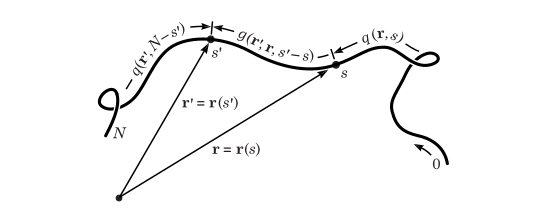
\includegraphics[width=15cm]{./figures/33.png}
\caption{解释了连续高斯链段密度-密度相关函数的合成公式(\ref{3.73})(仅最后一项)。轮廓长度-s的链端截面的统计权重$q(\mathbf{r},s)$在点$\mathbf{r}=\mathbf{r}(s)$处连接到传播子$g(\mathbf{r}^{'},\mathbf{r},s^{'}-s)$。传播子描述与长度为$s^{'}-s$的内部链段相关的统计权重,从$\mathbf{r}=\mathbf{r}(s^{'})$开始,结束于$r=r(s)$。最后“互补”链端截面的统计权重为$q(\mathbf{r},N-s^{'})$。}
\label{figure2}
\end{figure}

图\ref{figure2}描述了公式(\ref{3.72})的物理解释。该方程可用于计算具有势$w(\mathbf{r})$的连续高斯链段密度的二阶矩。虽然这类高阶密度相关函数的公式便于近似解析计算,但在高精度精度中应该避免。这是因为计算两点传播子(如$g(\mathbf{r},s,[w])$所付出的代价)。如果使用M个网格点或谱分量来求解空间自由度,请参见第3.6节,g的数值计算至少需要$M^2$算子。在三维模拟中, 使用这样的$O(M^2)$缩放的计算令人望而却步, 其中M大到$10^6-10^7$.
\subsubsection{应力算子(Stress operators)}
另一个重要的量是放置在不均匀环境中的聚合物链所产生的平均弹性应力。弹性应力算子可以定义为:
\begin{equation}\label{3.76}
\sigma(\mathbf{\mathbf{r}};[w,\epsilon])\equiv<\hat{\sigma}(\mathbf{r})>_{[w,\epsilon]}
\end{equation}
其中,单链平均是根据公式(\ref{3.47})计算的。用离散高斯链模型计算这个表达式的右边会产生两个不同的表达式,
\begin{align}\label{3.77}
\begin{split}
\sigma(\mathbf{r};[w,\epsilon])&=\frac{\int {\tilde{\sigma}}(\mathbf{r})~\exp[-\beta U(\mathbf{r}^{N+1})-\beta U_{el}(\mathbf{r}^{N+1})]~d\mathbf{r}^{N+1}}{\int \exp[-\beta U(\mathbf{r}^{N+1})-\beta U_{el}(\mathbf{r}^{N+1})]~d\mathbf{r}^{N+1}}\\&=\frac{\int \tilde{\sigma}(\mathbf{r})~\exp[-\beta U(\mathbf{r}^{N+1})-\beta U_{el}(\mathbf{r}^{N+1})]~d\mathbf{r}^{N+1}}{Q[w,\epsilon]~\int \exp[-\beta U_0(\mathbf{r}^{N+1})-\beta U_{el}(\mathbf{r}^{N+1})]~d\mathbf{r}^{N+1}}
\end{split}
\end{align}
第二个是最方便计算的。在最后一个表达式中插入微观应力运算符公式(\ref{3.11})的显式形式将导致:
\begin{equation}
\begin{aligned}\label{3.78}
\sigma_{\alpha \gamma}(\mathbf{r};[w,\epsilon])&=\frac{3k_BT}{b^2VQ[w,\epsilon]} \int (\mathbf{r}^{'}-\mathbf{r})_{\alpha} (\mathbf{r}^{'}-\mathbf{r})_{\gamma} \varPsi (\mathbf{r}^{'}-\mathbf{r};[\epsilon])\\&\times \sum_{j=0}^{N-1}q(\mathbf{r}^{'},N-j-1;[w,\epsilon])~q(\mathbf{r},j;[w,\epsilon])~d\mathbf{r}^{'}
\end{aligned}
\end{equation}
其中函数$\varPsi (\mathbf{r}^{'}-\mathbf{r};[\epsilon])$是在公式(\ref{3.14})中定义的。这个表达式可以通过先解公式(\ref{3.15})-(\ref{3.17})得到传播子$q(\mathbf{r},j;[w,\epsilon])$和配分函数$Q[w,\epsilon]$然后指定公式(\ref{3.78})中的被积和求和,其余运算可以数值计算出来。

在连续高斯链模型的基础上,导出了应力算子的类似表达式(Fredrickson,2002)。对于非均匀应变场,这个表达式是相当复杂的,因此不在这里再现。在均匀应变$\epsilon$的情况下,得到$^{19}$.
\begin{equation}\label{3.79}
\sigma(\mathbf{r};[w,\epsilon])=\frac{k_BTb^2}{3VQ[w,\epsilon]}\int_{0}^{N} q(\mathbf{r},s;[w,\epsilon])~\nabla \nabla q(\mathbf{r},N-s;[w,\epsilon])~ds
\end{equation}
应力算子的这个表达式表明,在空间变化的化学势$w(\mathbf{r})$存在下,弹性应力是各向异性的和非均匀的。应力各向异性是由沿链等高线积分的并矢量$q\nabla \nabla q$来表示的。泰勒和莫尔斯在研究嵌段共聚物中间相的线弹性性质时,推导出了密切相关的公式(Tyler and morse,2003a;Tyler and Morse,2003b)。方程(\ref{3.79})对于研究细观结构聚合物流体中链拉伸的不均匀分布特别有用。
